\documentclass{article}

\usepackage[utf8]{inputenc}
\usepackage{amsmath}
\usepackage{float}
\usepackage[top=1.5cm,bottom=1.5cm,left=1.5cm,right=1.5cm]{geometry}
\usepackage{graphicx}
\usepackage{enumerate}
\usepackage{listings}
\usepackage{color}
\definecolor{mycolor}{gray}{0.95}
\lstset{language=Matlab,breaklines = true, backgroundcolor=\color{mycolor}}
\usepackage[usenames,dvipsnames]{xcolor}
\usepackage{multicol}

\begin{document}
\begin{center}
{\Large \textbf{Utilización del Arduino para controlar motores de paso por medio del flasheo de GRBL}}\\
\vspace{0.3cm}
\textit{Alfredo Ricci, Juan Andrés Urrea}
\end{center}
\begin{multicols}{2}
\textbf{Resumen- Este informe busca mostrar la totalidad del procedimiento realizado para configurar un computador y un arduino como controladores para motores de paso. Se centra en la instalación del software necesario tanto en su utilización una vez esto se completa, al igual que la posterior creación y utilización de una interfaz gráfica en Matlab como herramienta para el usuario. De esta forma, explica el procedimiento de instalación y configuración, sirviendo a la vez como un tutorial para repetir este procedimiento.}

{\centering \section{Introducción}}
Dada la necesidad de tener un conocimiento previo del manejo tanto manual como automatizado de los motores utilizados para el proyecto \textbf{Mechanical Scanner}, se ideó la estrategia de reproducir esta situación a pequeña escala, usando motores de paso para luego conectarlos a un Arduino flasheado con GRBL y aprender, desde cero, los procesos necesarios para transmitir órdenes de trayectorias desde un computador hasta los motores de paso utilizados. De esta forma, la construcción exitosa de este montaje y la capacidad de controlar detalladamente estos dispositivos por medio de un manejo apropiado del software permitirá obtener este conocimiento previo a la llegada y utilización del \textbf{Mechanical Scanner}.

{\centering \section{Montaje Utilizado}}
A continuación se presenta el diagrama que describe el montaje de conexión realizado entre el arduino, el cnc shield, los drivers, motores y computador como base de control.

\begin{figure}[H]
\centering
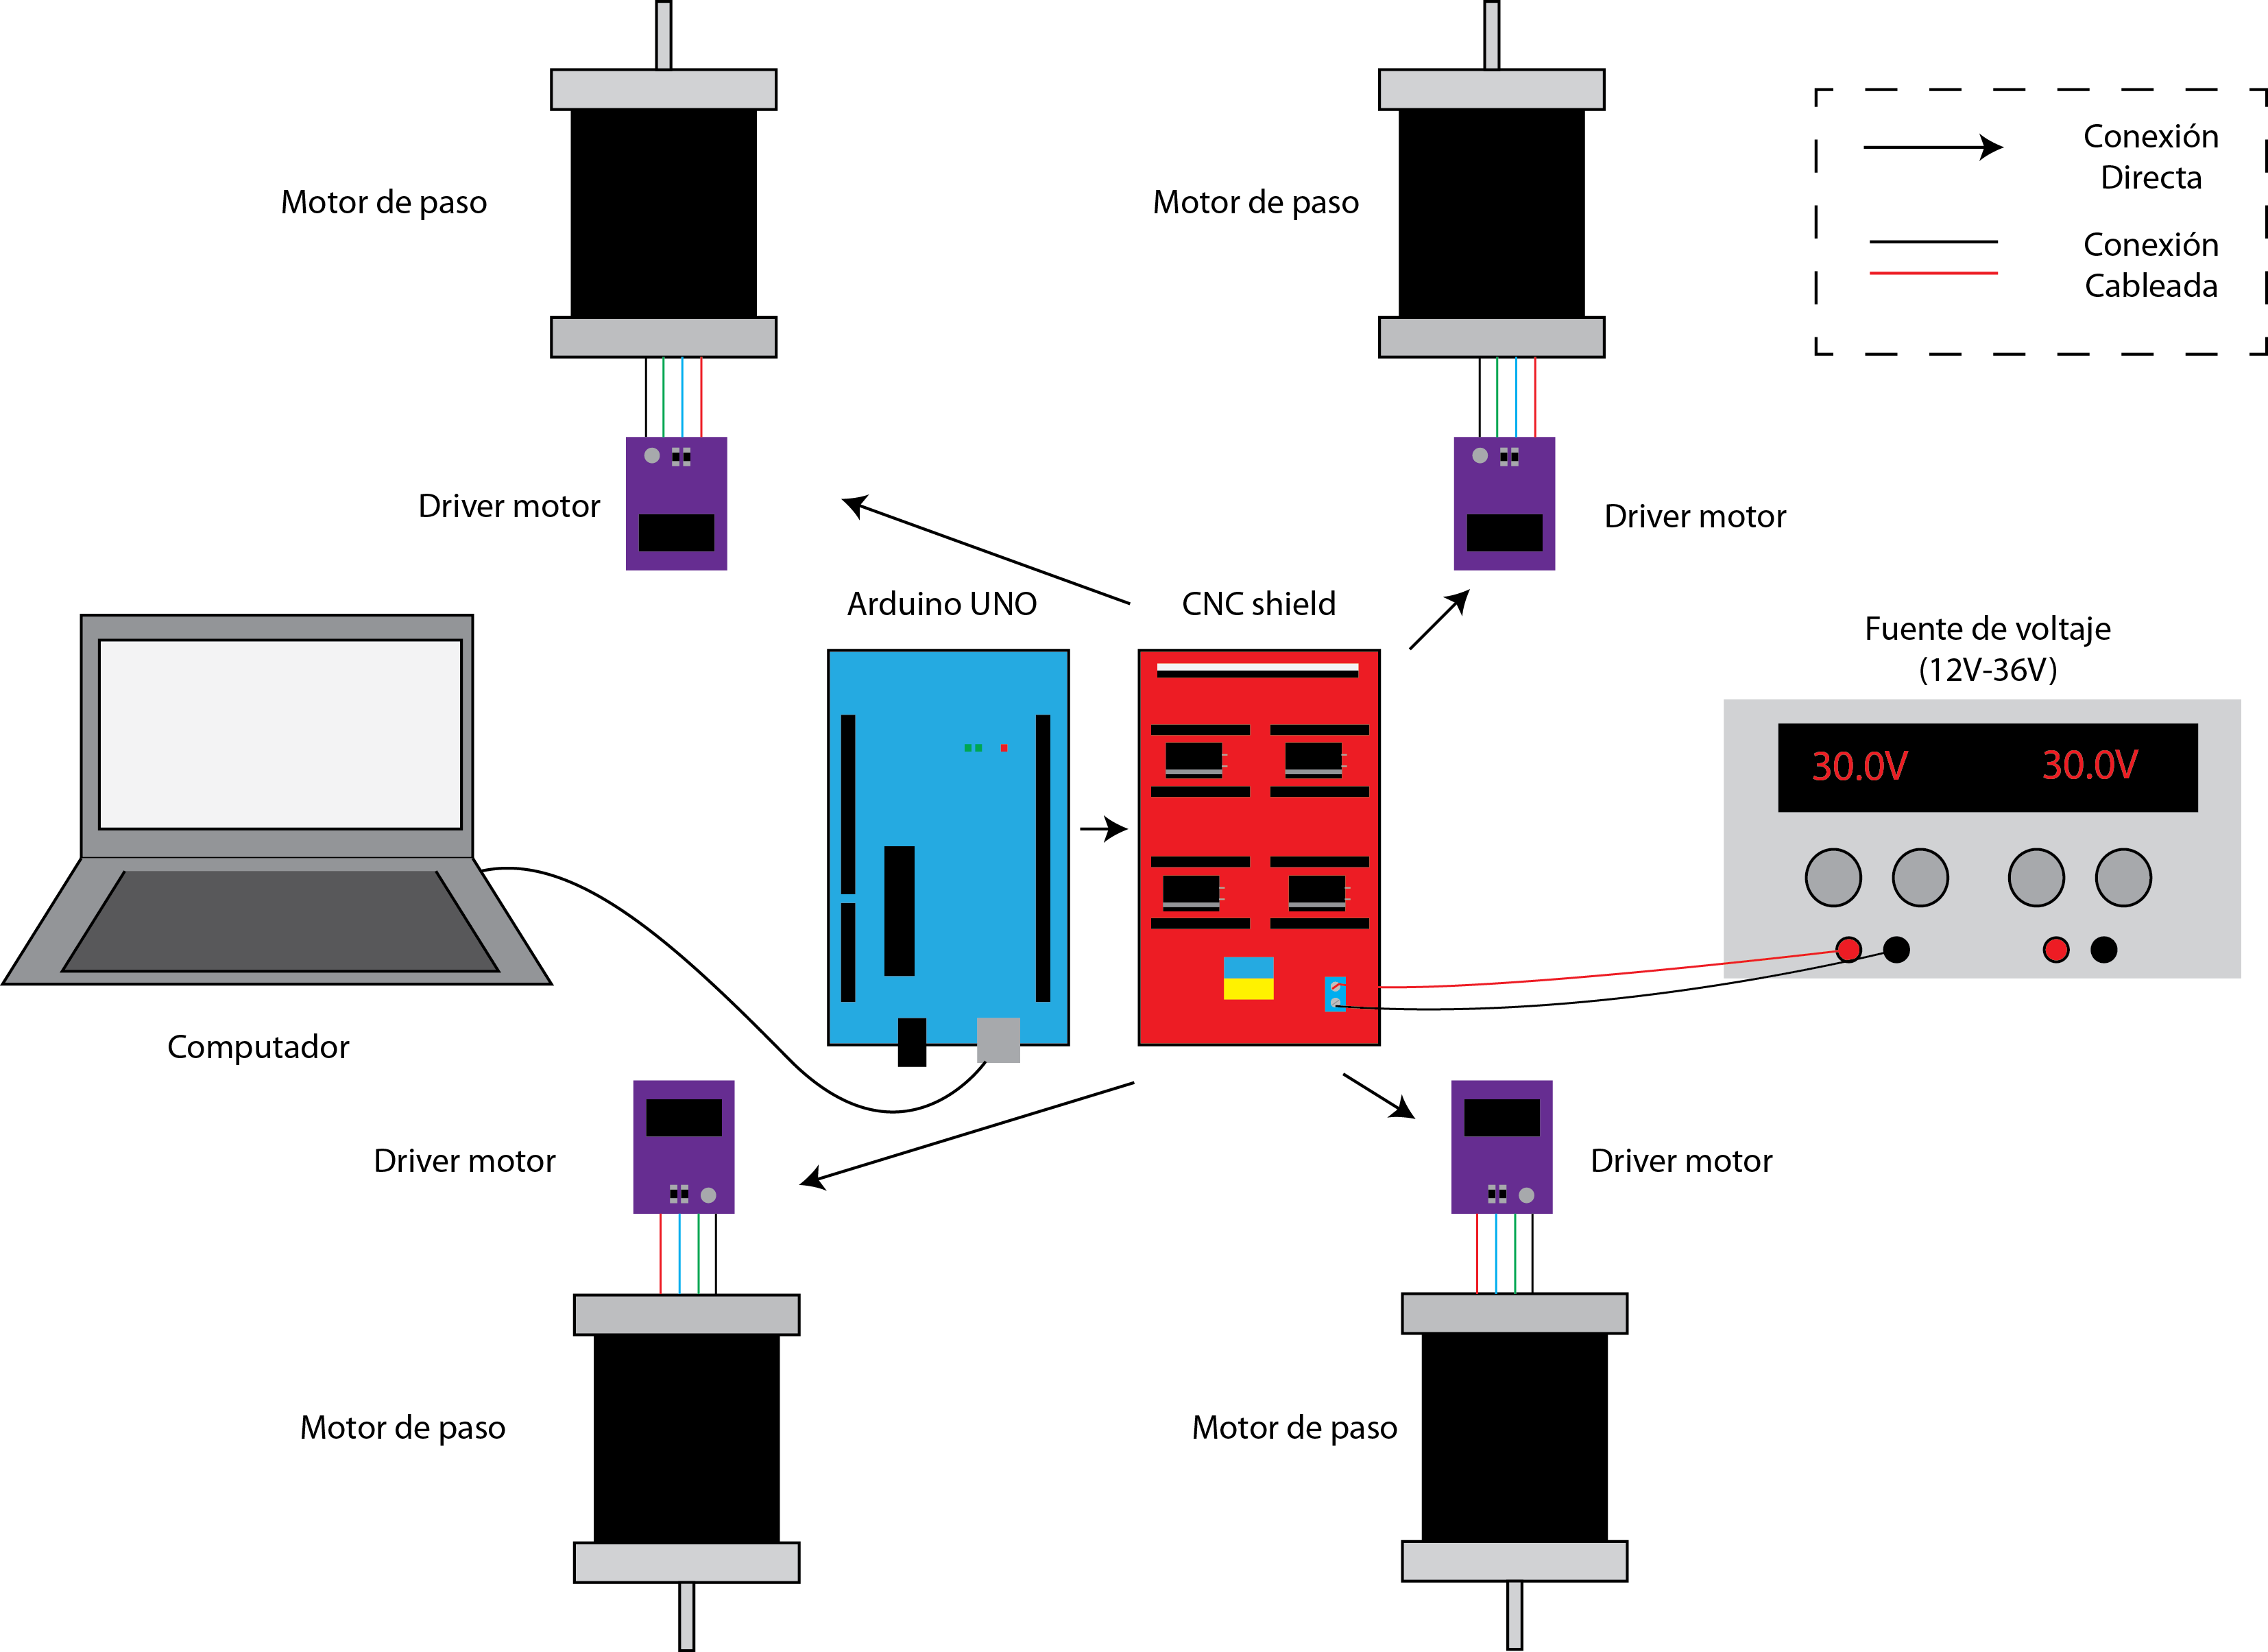
\includegraphics[width=0.5\textwidth]{Montaje.png}
\label{fig:montaje}
\end{figure}

{\centering \section{Manejo de Software}}
{\centering \subsection{Instalación de Software Utilizado}}
Antes de la explicación detallada acerca del proceso de instalación, se enuncian a continuación los diferentes programas y software utilizados:
\begin{itemize}
\item \textbf{GRBL}\\
\begin{itemize}
\item Versión: 0.9
\end{itemize}
GRBL es un controlador de movimiento disponible para funcionar con Arduino, escrito enteramente en \textit{C}, que sirve como alternativa al control por puerto paralelo. Este software permite utilizar archivos escritos en \textit{GCode} para diseñar trayectorias a seguir, de manera que estos se convierten en instrucciones para el Arduino, por medio de la instalación de GRBL, que luego son enviadas a la tarjeta controladora CNC.

\item \textbf{Arduino UNO}\\
\begin{itemize}
\item Versión 1.6.5
\end{itemize}
Software que funciona como interfaz para controlar el dispositivo arduino desde un computador. Puede instalarse directamente desde la página web de Arduino. Software programado en Java, permite la creación de código que luego es subido directamente al dispositivo Arduino.

\end{itemize}
\begin{center}
\textbf{Instalación del Software Requerido}
\end{center}
Una cez se sabe cual es el software requerido, se presenta ahora el proceso detallado de instalación de estos. Cabe notar que el proceso mostrado a continuación se realizó tanto en Linux como en Mac. Esto con la finalidad de utilizar los procedimientos más sencillos que ofrece cada sistema operativo. Para este caso, el flasheo de GRBL al Arduino se realizó desde Linux, mientras que la construcción y envío de GCode al Arduino se realizó desde Mac. Estas diferencias se enunciarán en cada paso.

\begin{enumerate}
\item \textbf{Revisión de Librerías de Instalación Linux}\\
Cuando se trabaja con Linux, especificamente la distribución Ubuntu 14.04 "Trusty", se debe realizar una verificación de librerías que permiten la instalación correcta de paquetes. Dicho proceso se puede realizar con los siguientes comandos de instalación en la terminal. En caso de que ya se encuentren actualizadas, en la terminal esto será notificado. En caso de que no, se instalarán.
\begin{lstlisting}
sudo apt-get install ruby
sudo apt-get install avrdude
\end{lstlisting}

\item \textbf{Descargar GRBL y Flashearlo}\\
Ahora, es necesario descargar todo lo relacionado a GRBL. Esto se puede realizar desde GitHub, en el enlace [1]. Para hacer esto, se recomienda, si es que es la primera vez que se trabaja con esta herramienta, seleccionar la opción \textbf{Download Zip} en la parte derecha de la página.
\begin{figure}[H]
\centering
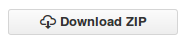
\includegraphics[width=0.3\textwidth]{BotonDescarga.png}
\label{fig:Boton}
\end{figure}

El archivo zip descargado debe luego ser descomprimido en una carpeta cuya localización resulte fácil de recordar. Debido a como está en GitHub, el archivo descargado se llamará \textbf{grbl-edge}. Para continuar este procedimiento, se abre ahora la carpeta recién descargada, buscando el archivo llamada \textbf{Makefile}, el cual debe ser después abierto con un editor de texto de preferencia personal, en este caso \textbf{Gedit}, editor de texto predeterminado de Ubuntu.

\begin{figure}[H]
\centering
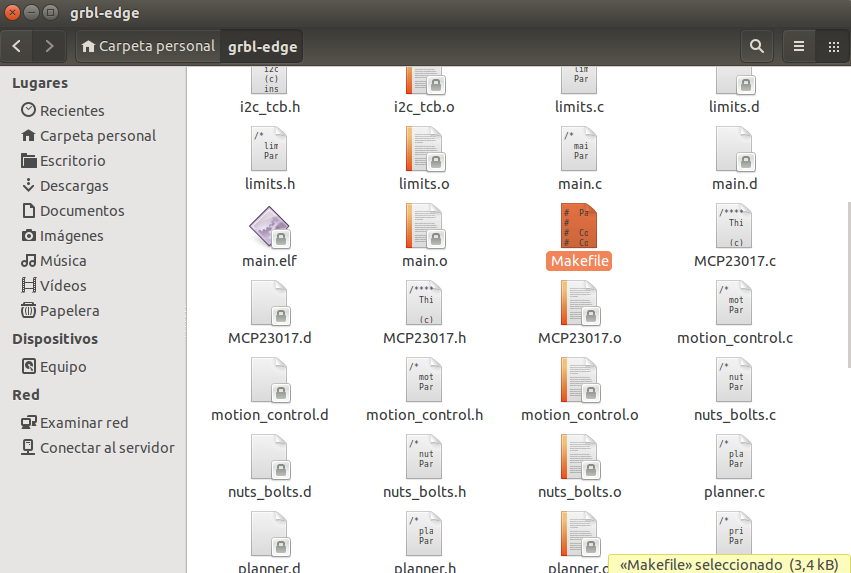
\includegraphics[width=0.4\textwidth]{Carpeta.png}
\label{fig:Carpeta}
\end{figure}

Una vez abierto este archivo, se busca la línea que empieza por la palabra \textit{PROGRAMMER}, para reemplazarla por lo siguiente:
\begin{lstlisting}
PROGRAMMER = -c stk500v1 -P /dev/ttyACM0 -b 115200 
\end{lstlisting}
El archivo luego debe guardarse para actualizar y aplicar los cambios realizados. Una vez se hace esto, se debe abrir una terminal nueva. Esto para aprovechar las ventajas de control que esta aplicación ofrece. Desde esta se debe acceder a la carpeta \textbf{grbl-edge} creada anteriormente. Aunque la apariencia de la terminal depende sustancialmente de la configuración en cada equipo, para este caso específico se obtiene la siguiente ventana:

\begin{figure}[H]
\centering
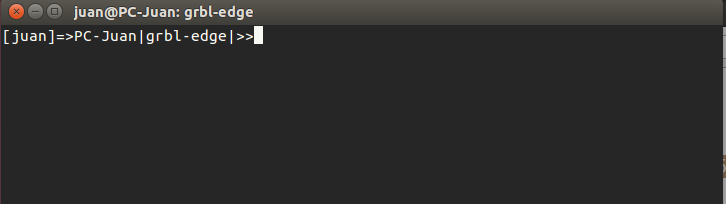
\includegraphics[width=0.45\textwidth]{Terminal.png}
\label{fig:Carpeta}
\end{figure}

Una vez dentro de este entorno, se utiliza las siguientes líneas de código, para inicializar el archivo \textbf{make} dentro de la carpeta.
\begin{lstlisting}
sudo make clean
sudo make
\end{lstlisting}
Realizar esto causará que aparezcan varias notificaciones en la terminal, las cuales sirven únicamente para informar de los procesos completados. Para finalizar este procedimiento, solo resta flashear GRBL al Arduino. Para hacer esto, se debe conectar el Arduino al computador en uso. Luego de hacer esto, se ejecuta en la terminal la siguiente línea de código.
\begin{lstlisting}
sudo make flash
\end{lstlisting}
Esta línea instalará GRBL en el arduino, tras de lo cual se puede desconectar del computador y usar como controlador de movimiento de ahora en adelante.
\end{enumerate}
{\centering \section{Construcción de la Interfaz Gráfica en Matlab}}
Una vez se han instalado los programas necesarios para la realización del flasheo y este mismo se ha realizado, resulta ahora necesario la construcción de una interfaz gráfica y funcional desde Matlab que permita al usuario la creación de barridos de forma manual, el seleccionamiento de barridos predeterminados y en general el control del movimiento por medio de parámetros, a la vez que el recibimiento de una retroalimentación de posiciones constante. Con este objetivo se comienza entonces este procedimiento, empezando con la utilización de la función \textbf{GUIDE} de Matlab, ejecutando el siguiente comando en la consola:
\begin{lstlisting}
>>guide
\end{lstlisting}
Este comando abre herramienta de creación de interfaz gráfica de Matlab, la cual comienza con el plano básico donde es posible insertar distintos tipos de elementos como botones, cuadros de texto editables, menus de despliegue, etc...A continuación se presentan las ventanas emergentes que dan comienzo a la creación de la interfaz gráfica.

\begin{figure}[H]
\centering
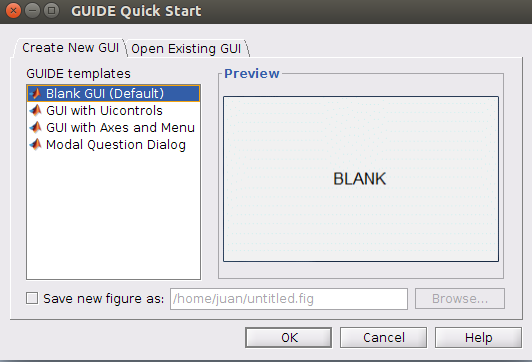
\includegraphics[width=0.45\textwidth]{GuideNuevo.png}
\label{fig:guide1}
\caption{Selección de Formato}
\end{figure}

\begin{figure}[H]
\centering
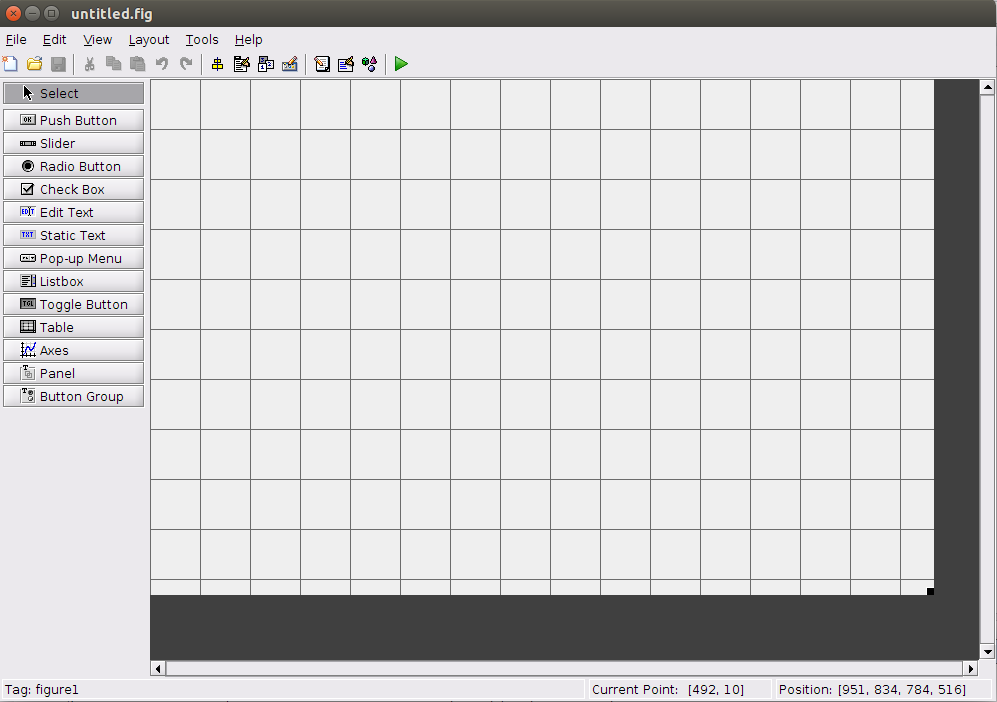
\includegraphics[width=0.45\textwidth]{GuidePlano.png}
\label{fig:guide2}
\caption{Ventana GUI nueva}
\end{figure}
En la figura \ref{fig:guide1} se observa la selección de plantilla que puede utilizarse para la construcción de una nueva interfaz. Para este caso se selecciona la opción \textit{Blank GUI (Default)}, puesto que no se busca partir de una plantilla predeterminada. Es posible también selecionar la casilla \textbf{Save new figure as}, de manera que se guarde desde ese momento la nueva figura creada. De hacer esto, se guardará en la carpeta deseada como archivo \textbf{.fig}, el cual puede ser modificado desde la opción \textit{guide} nuevamente cuando sea necesario.

Una vez se ha dado la opción \textbf{OK} y se ha elegido la plantilla en blanco, se despliega la ventana mostrada en la figura \ref{fig:guide2}, donde es posible comenzar la construcción de la interfaz deseada. Para trabajar específicamente con el modelo planeado para esta interfaz, mostrado a continuación, se exploran únicamente las opciones y herramientas que sirven para la creación de esta, encontrándose un tutorial más detallado de las demás opciones en [1]. \textbf{MONTAR FOTO}\\
A partir del modelo mostrado, se procede, inicalmente, a construir la estética de la interfaz, proceso que consiste en el solo posicionamiento de cada elemento dentro de la interfaz, sin trabajar aún en las funciones que cada uno cumple. Esto se hace seleccionando cada item mostrado a la izquierda en la figura \ref{fig:guide2} y llevándolo hasta la posición deseada. Esto se hace entonces con los elementos correspondientes a \textit{Push Button}, \textit{Static Text}, \textit{Edit Text}, \textit{Pop-Up Menu} y \textit{Check Box}. A continuación se enuncian brevemente las características de cada uno:
\begin{itemize}
\item \textbf{Push Botton:} Corresponde a un botón en la interfaz, de manera que al pulsarse se realiza algún procedimiento correspondiente.
\item \textbf{Static Text:} Corresponde a un cuadro de texto que puede ser editado por funciones de la interfaz mas no por el usuario, usado para mostrar resultados esencialmente de respuesta.
\item \textbf{Edit Text:} Corresponde a un cuadro de texto que puede ser editado por el usuario, de manera que la interfaz puede recibir como parámetro para funciones el valor ingresado aquí.
\item \textbf{Pop-Up Menu}: Corresponde a un menu desplegable que ofrece opciones que han sido definidas previamente en la construcción de la interfaz, de manera que la selección de cada opción conlleva a la realización de un procedimiento distinto.
\item \textbf{Check Box:} Corresponde a una casilla de selección con la posibilidad de ser marcada o no. Este estado definirá entonces una condición para la realización de procesos internos de la interfaz.
\end{itemize}
Una vez se ha posicionado cada elemento, es posible ahora editar el nombre con el que será identificado dentro de las funciones internas de la interfaz, a la vez que el texto que se ve sobre el en la estética de la interfaz. Para realizar este procedimiento, se da click derecho sobre cada elemento y se selecciona la opción \textbf{Property Inspector}, donde se muestran entonces las distintas propiedades editables disponibles para cada tipo de elemento. Para el procedimiento aquí realizado,  resulta únicamente necsario la edición de los campos \textbf{Tag} y \textbf{String}, los cuales representan el nombre bajo el cual se identifica el elemento dentro de las funciones de la interfaz y el texto que se ve sobre el elemento en la interfaz, respectivamente. El resultado de este procedimiento se muestra a continuación:

\begin{figure}[H]
\centering
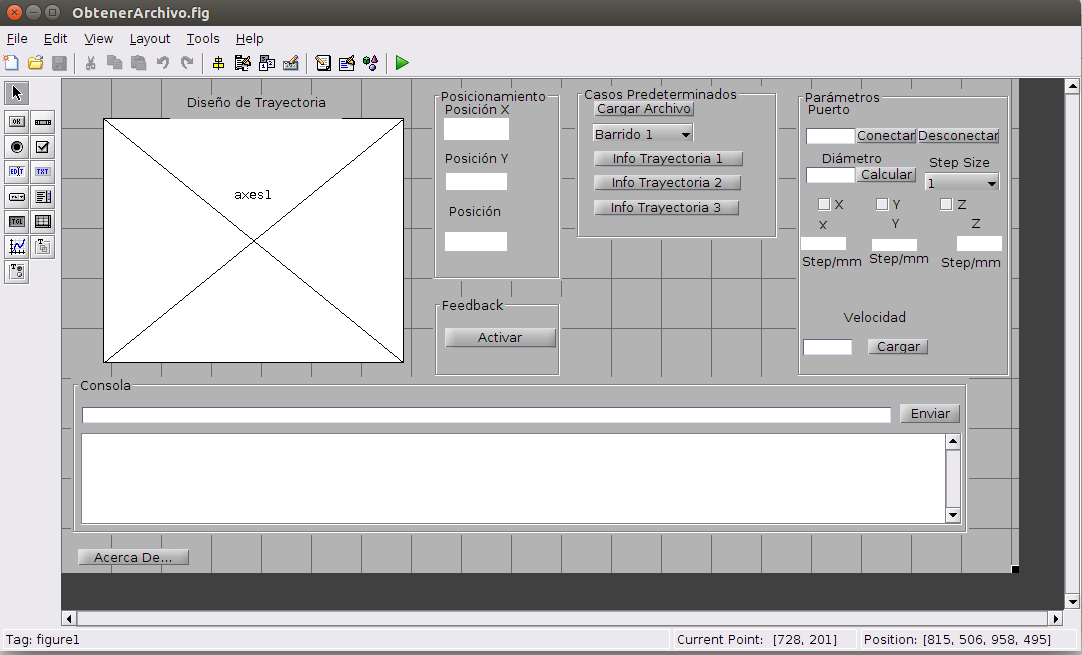
\includegraphics[width=0.48\textwidth]{GuideCompleto.png}
\label{fig:guide3}
\caption{Interfaz construida en GUI}
\end{figure}
Cabe notar la utilización del elemento \textbf{Panel}, el cual sirve únicamente como herramienta de estética para crear divisiones dentro de la interfaz para crear orden.La creación del título correspondiente a cada uno se realiza de igual forma en la ventana correspondiente de \textit{Property Inspector}. Con este procedimiento se ha finalizado ya la etapa estética de la construcción de la interfaz, por lo que se procede ahora a la construcción de las funciones internas que dan a cada elemento utilizado un funcionamiento o relación con otros según se necesita en la aplicación. Para comenzar a construir dichas funciones, se establecen entonces las diferentes funciones que se necesitan de primera mano por parte del usuario, al igual que aquellas que deben crearse internamente como consecuencias de estas. Se enuncian a continuación las funciones generales que la interfaz debe cumplir para dar al usuario control sobre el movimiento de los motores, al igual que información acerca de la posición de estos en todo momento.

\begin{center}
\textbf{Requerimientos Funcionales}
\end{center}
A continuación se enuncian los requerimientos funcionales generales que debe cumplir la interfaz como medio de comunicación entre el usuario y el montaje de los motores.
\begin{enumerate}[(a)]
\item Permitir al usuario mandar código G que defina el movimiento deseado de manera manual.
\item Permitir al usuario enviar una trayectoria predeterminada a realizar, ya sea de un archivo de código G escrito previamente o una trayectoria construida por la interfaz por medio de parámetros de entrada.
\item Proveer al usuario una retroalimentación constante tanto como verificación de lo que fue enviado por este tanto de la posición actual dada por el montaje, todo por medio de una consola en tiempo real.
\item Permitir al usuario modificar parámetros del montaje para los cálculos internos de GRBL, como lo son el diámetro de las ruedas utilizadas, el $\frac{Step}{mm}$ en cada dirección, etc...
\item Permitir al usuario definir manualmente el puerto serial donde se trabajará la conexión, de manera que se pueda establecer la relación entre la interfaz de Matlab y el montaje.
\end{enumerate}

\begin{center}
\textbf{Generalidades acerca del envío de comandos a GRBL Versión 0.9}
\end{center}
Cada versión disponible actualmente de GRBL cuenta con una serie de comandos específicamente designados para que, al ser enviados por puerto serial al montaje de CNC, devuelva información específica de este o modifique un parámetro de su movimiento. La lista entera se puede encontrar en el repositorio oficial de GitHub[2], sin embargo a continuación se enuncian los que son utilizados en la construcción de la interfaz de usuario y el código que define sus funciones:
\begin{itemize}
\item \textbf{$\$ 100$}\\
Al introducir este comando por puerto serial y enviarlo a GRBL igualado a un valor numérico, este valor se tomará como el $\frac{Step}{mm}$ en la dirección X. Un ejemplo es:
\begin{lstlisting}
>>$100=25.6
\end{lstlisting}
Donde el $\frac{Step}{mm}$ tomará el valor de 25.6.

\item \textbf{$\$ 101$}\\
Al introducir este comando por puerto serial y enviarlo a GRBL igualado a un valor numérico, este valor se tomará como el $\frac{Step}{mm}$ en la dirección Y. Un ejemplo puede ser el mismo que el mostrado para la dirección X, escribiendo ahora $\$ 101$.

\item \textbf{$\$ 102$}\\
Al introducir este comando por puerto serial y enviarlo a GRBL igualado a una valor numérico, este valor se tomará como el $\frac{Step}{mm}$ en la dirección Z. El ejemplo es igual a los mostrados anteriormente.
\end{itemize}

Teniendo definidos estos requerimientos, se procede entonces a construir el código dentro del archivo \textbf{.m} que se creó simultáneamente a la creación del archivo \textbf{.fig}. Para hacer esto, se comienza entonces con todo lo relacionado a la selección de archivos externos o trayectorias predeterminadas. Esto corresponde al panel denominado \textit{Casos Predeterminados}. Se muestra a continuación el código detallado y documentado para cada aspecto necesario de este grupo de funciones:
\begin{itemize}
\item \textbf{Cargar Archivo}\\
Esta función permite al usuario cargar al montaje un archivo escrito en código G de manera que cada línea se envíe por consola al montaje. Para lograr hacer esto, el archivo seleccionado se importa y su contenido se almacena tempiralmente línea por línea en una variable, siendo este luego enviado al puerto serial.
\begin{lstlisting}
function Cargar_Callback(hObject, eventdata, handles)
%Se crea la ventana para cargar archivos de tipo .g. 
[Filename Path]=uigetfile({'*.g'},'Abrir archivo');
%Se establecen los casos para actuar segun lo seleccionado.
if isequal(Filename,0)
    return
else
    %Se recibe el archivo y su contenido es leido, almacenado y enviado.
end
\end{lstlisting}
\item \textbf{Cargar Trayectoria Predeterminada}\\
Esta función permite al usuario desplegar un menú en lista donde se muestran las distintas trayectorias predeterminadas que pueden ser utilizadas para el montaje. De seleccionar una de la lista, en el eje denominado \textit{Axes}, mostrado en la figura \ref{fig:guide3}, se debe mostrar la imagen de esta trayectoria, a la vez que se despliega una ventana emergente para ingresar los parámetros geométricos que definen cada trayectoria.\\
\textbf{En Proceso:} Debido a que la totalidad de esta función no se ha finalizado, solo se muestran a continuación las acciones parciales que realiza hasta ahora. estas son la aparición de una foto que identifica cada trayectoria. Apenas se tengan los scripts que definen cada trayectoria según parámetros, se actualizará el código correspondiente a continuación.
\begin{lstlisting}
function Predet_Callback(hObject, eventdata, handles)
%Definir los distintos valores que pueden ser adoptados en la seleccion.
fun = get(hObject,'Value');
    switch fun
    %Definir cada caso y la accion que se toma en cada uno.
        case 1
        %Se muestra en el eje de imagenes la imagen correspondiente a cada trayectoria.
            a = imread('A.png');
            imshow(a);
            %Se despliega la ventana emergente para ingresar los parametros de cada trayectoria.
            x=inputdlg({'Parametro A','Parametro B'},'Parametros');
            %x sera una celda de dos elementos.
            params=cell2mat(x);
            %params es un arreglo con estos valores. Posteriormente sera posible manipularlos para la creacion de la trayectoria.
        case 2
            b = imread('B.jpg');
            imshow(b);
        case 3
            c = imread('C.png');
            imshow(c);
                
    end
guidata(hObject,handles);
\end{lstlisting}
\item \textbf{Dar Información acerca de cada Trayectoria}\\
Esta función permite al usuario obtener información general acerca de cada una de las trayectorias predeterminadas disponibles en la forma de mensajes informativos en ventanas emergentes, activadas por el botón correspondiente. Esta herramienta viene definida entonces para tres botones distintos; \textbf{Info Trayectoria 1}, \textbf{Info Trayectoria 2} y \textbf{Info Trayectoria 3}. Por le momento, dado que no se han definido estas trayectorias, se muestra un mensaje genérico para la trayectoria 1, mientras que permanece siendo posible editar los tres emnsajes una vez se construyan correctamente las trayectorias.
\begin{lstlisting}
function Info1_Callback(hObject, eventdata, handles)
msgbox('Esta trayectoria realiza un barrido dado por la geometria mostrada en la figura. Para construirlo, el usuario debe dar los parametros requeridos.','Trayectoria 1');
%Info de la trayectoria 1.
\end{lstlisting}
\end{itemize}
Ahora se continua con el panel relacionado a la modificación de los parámetros de conexión y configuraciones de los motores utilizados, como lo son la selección del puerto serial donde se encuentra conectado el Arduino, los $\frac{Step}{mm}$ en cada dirección, la velocidad de los motores, etc... Para lograr todas estas funcionalidades, se implementó el código mostrado y documentado a continuación.
\begin{itemize}
\item \textbf{Selección de Puerto Serial}\\
Esta función permite al usuario seleccionar el puerto serial al cual quiere realizar la conexión y hacerla, haciendo uso del botón \textbf{Conectar}. De manera similar, permite cerrar dicha conexión con el botón \textbf{Desconectar}.
\begin{lstlisting}
function Connect_Callback(hObject, eventdata, handles)
global s; %Se declara s como una variable global para que todas las funciones puedan acceder a esta si la necesitan.
puerto=handles.Port; %Se establece la variable local puerto como lo que el usuario escribe en el campo de Puerto.
s=serial(puerto); %Declarar puerto serial.
fopen(s); %Abrir la conexion al puerto serial.
\end{lstlisting}
\item \textbf{Desconectar}\\
Esta función permite cerrar la conexión serial previamente establcida con el puerto seleccionado, haciendo referencia a la variable local que lo contiene.
\begin{lstlisting}
function Disconnect_Callback(hObject, eventdata, handles)
global s; %Permite modificar la variable s.
fclose(s); %Cierra la conexion al puerto serial.
\end{lstlisting}
\item \textbf{Calcular el $\frac{Step}{mm}$ en cada eje}\\
Esta función permite determinar el $\frac{Step}{mm}$ en cada eje de dirección, basándose en parámetros de entrada como lo son el diámetro de las ruedas o poleas a utilizar y el \textit{Step Size}, seleccionado de una lista desplegable, al igual que seleccionando la dirección que se desea trabajar. El código implementado para lograr esto se muestra documentado a continuación. Ya que este proceso requiere la utilización de varios campos de texto junto con botones, se muestran las distintas funciones separadas.
\begin{lstlisting}
function checkbox1_Callback(hObject, eventdata, handles)
%Se define la funcion del checkbox de X.
global chuleadoX; Se torna la variable en global para poder referenciarla desde otras funciones.
%En caso de estar marcado, la variable gobal toma el valor 1, en caso contrario toma el valor 0.
if(get(hObject,'Value')== get(hObject,'Max'))
    chuleadoX=1;
else
    chuleadoX=0;
end

%Las funciones para los dos checkbox restantes tiene la misma estructura, variando unicamente la variable global que se modifica.

function checkbox2_Callback(hObject, eventdata, handles)
global chuleadoY;
if(get(hObject,'Value')==get(hObject,'Max'))
    chuleadoY = 1;
else
    chuleadoY=0;
end

function checkbox3_Callback(hObject, eventdata, handles)
global chuleadoZ;
if(get(hObject,'Value')==get(hObject,'Max'))
    chuleadoZ=1;
else
    chuleadoZ=0;
end
    
function Diameter_Callback(hObject, eventdata, handles)
%La funcion define como utilizar el parametro de entrada del valor de diametro. 
Val=get(hObject,'String'); %Se recibe el parametro de tipo String.
NewVal=str2double(Val); %Se convierte el valor en un caracter numerico decimal.
handles.Diameter=NewVal; %Se guarda el valor de la variable.
guidata(hObject,handles); %Se guarda la variable en la informacion de la funcion.

function Pasos_Callback(hObject, eventdata, handles)
global Step; %Se declara la variable global para ser accesible por otras funciones.
fun=get(hObject,'Value')
%Se declara una variable local cuyo valor esta dado por las opciones del menu desplegable.
    switch fun
    %La variable global Step tomara el valor correspondiente al Step Size deseado por el usuario.
        case 1
           Step = 1;
        case 2
            Step = 1/2;
        case 3
            Step = 1/4;
        case 4
            Step = 1/8;
        case 5
            Step = 1/16;
        case 6
            Step = 1/32;
    end
    guidata(hObject, handles);
    
function Calcular_Callback(hObject, eventdata, handles)
%Se importan las variable globales definidas en funciones anteriores, que son necesarias para el calculo del Step/mm.
global Step; 
global chuleadoX;
global chuleadoY;
global chuleadoZ;
global s;
global consola;

%Primero, se definen excepciones generales, de manera que sea necesario modificar de a una variable a la vez, por lo que habra un mensaje de error en caso de seleccionar mas de una en los checkbox, a la vez que existira un error si no se selecciona ninguna para modificar.
if((chuleadoX == 1) && (chuleadoY == 1) && (chuleadoZ == 1))
    errordlg('Se debe seleccionar solo una coordenada para modificar.','Error de Parametros');
end
if(chuleadoX == 1 && chuleadoY ==1 && chuleadoZ == 0)
    errordlg('Se debe seleccionar solo una coordenada para modificar.','Error de Parametros');
end
if(chuleadoX == 0 && chuleadoY ==1 && chuleadoZ == 1)
    errordlg('Se debe seleccionar solo una coordenada para modificar.','Error de Parametros');
end
if(chuleadoX == 1 && chuleadoY ==0 && chuleadoZ == 1)
    errordlg('Se debe seleccionar solo una coordenada para modificar.','Error de Parametros');
end
if(chuleadoX == 0 && chuleadoY ==0 && chuleadoZ == 0)
    errordlg('Se debe seleccionar una coordenada para modificar.','Error de Parametros');
end

%Cuando no se presenta ningun error, se procede a realizar el calculo para la variable seleccionada.
if(chuleadoX == 1 && chuleadoY==0 && chuleadoZ==0)%Condiciones de los checkbox.
%Se calcula el step por mm y se muestra, para luego enviarlo al CNC.
    calculo = (200*(1/(Step))/(pi*handles.Diameter));
    set(handles.PasosX,'String',calculo);
    fprintf(s,strcat('$100=',num2str(calculo)));
    lectura=fscanf(s,'%s'); %Leer el feedback
    consola = strvcat(consola,strcat('>>>','$100=',num2str(calculo)),lectura);
    set(handles.Resultado,'String',consola);
end

%Este mismo procedimiento se repite para los casos en los cuales la coordenada Y o Z hayan sido seleccionadas.

if(chuleadoY==1 && chuleadoX==0 && chuleadoZ==0)
    calculo = (200*(1/(Step))/(pi*handles.Diameter));
    set(handles.PasosY,'String',calculo);
    fprintf(s,strcat('$101=',num2str(calculo)));
    lectura=fscanf(s,'%s'); %Leer el feedback.
    consola = strvcat(consola,strcat('>>>','$101=',num2str(calculo)),lectura);
    set(handles.Resultado,'String',consola);
end

if(chuleadoZ==1 && chuleadoX==0 && chuleadoY==0)
    calculo=(200*(1/(Step))/(pi*handles.Diameter));
    set(handles.PasosZ,'String',calculo);
    fprintf(s,strcat('$102=',num2str(calculo)));
    lectura=fscanf(s,'%s'); %Leer el serial en formato string.
    consola = strvcat(consola,strcat('>>>','$102=',num2str(calculo)),lectura);
    set(handles.Resultado,'String',consola);
end

function Speed_Callback(hObject, eventdata, handles)
%Esta funcion define como se recibe y almacena el parametro de velocidad.
Val=get(hObject,'String'); %Recibir el parametro de la velocidad como String.
handles.Speed=Val; %Guardar la variable temporal para ser referenciada por otras funciones.
%El resto de esta funcion sigue en construccion.
guidata(hObject,handles);
\end{lstlisting}
\end{itemize}
Ahora, se procede a construir todo lo correspondiente al Panel de \textbf{Consola}, el cual contiene tres elementos principales:
\begin{enumerate}[(a)]
\item La barra de texto editable donde se introducen los comandos de código G o de edición de parámetros de manera manual por el usuario.
\item El botoón denominado \textbf{Enviar}, el cual envía por medio de puerto serial dichos comandos introducidos.
\item La celda de texto no editable que va mostrando el feedback de confirmación que devuelve el CNC, al igual que muestra el historial de comandos enviados por el usuario.
\end{enumerate}
El código específicamente implementado para dar funcionalidad a estos tres elementos se muestra documentado a continuación.
\begin{lstlisting}
function Comandos_Callback(hObject, eventdata, handles)
Val=get(hObject,'String'); %Recibir el comando escrito en la celda de texto editable.
NewVal = char(Val); %Convertir a arreglo de tipo Char.
handles.Comandos=NewVal; %Guardar el contenido dentro de la informacion de la funcion.
guidata(hObject,handles);

function Enviar_Callback(hObject, eventdata, handles)
global s; %Importar la variable global que define el puerto serial.
global consola; %Importar la variable global que contiene el historial de comandos enviados.
input = handles.Comandos; %Importar arreglo de Char.
consola = strvcat(consola,strcat('>>',input));  %Actualizar la variable Consola con los comandos enviados.
set(handles.Resultado,'String',consola); %Mostrar en la celda de texto de feedback la nueva variable consola actualizada.
fprintf(s,input); %Enviar comando directamente por puerto serial.
\end{lstlisting}
A continuación, se procede entonces a la construcción de las herramientas que permiten a la interfaz recibir la retroalimentación dada por el CNC tras el envío de comando por parte del usuario, de manera que la consola muestre no solo los comandos utilizados previamente, sino también las respuestas del CNC a estos, a manera de confirmar su correcto recibimiento o enterarse de cualquier error que pudiese ocurrir en el envío. Para realizar este procedimiento, se realiza una lectura periódica del puerto serial y los resultados obtenidos se imprimen automáticamente en la consola, utilizando para esto el código mostrado a continuación.
\begin{lstlisting}
function feedbackButton_Callback(hObject, eventdata, handles)
global consola;
global s;
limite = 1000; %Tiempo en segundos durante el cual se realiza la lectura.
contador = 0; %Contadora.
borrar = 0; %Decidir cuando borrar.
while(contador < limite)
    lectura=fscanf(s,'%s'); %Leer el serial en formato string.
    consola = strvcat(consola,lectura); %Anadir a variable de consola.
    set(handles.Resultado,'String',consola); %Mostrar en consola de interfaz.
    contador = contador +1;
    pause(0.1); %El descanso.
end
\end{lstlisting}
La función definida y documentada anteriormente se ejecuta cuando el botón \textbf{Activar} del panel \textbf{Feedback} se oprime, de manera que paralelemanete a cualquier acción que se esté realizando, se realiza también una lectura constante del serial cada 0.1 segundos hasta completar 1000 lecturas consecutivas.  Adicionalmente a esta función, se crea una código que complementa cada función que envía comandos al puerto serial del CNC, de manera que la respuesta de este a estos códigos es leída e impresa en la consola de la interfaz. Dicho complemento se muestra a continuación:
\begin{lstlisting}
lectura=fscanf(s,'%s'); %Leer el feedback.
\end{lstlisting}
Esta línea de código se coloca justo despues de la línea que incluye el comando \textbf{fprintf()}, de manera que tras recibir el código enviado, el CNC envía una respuesta que la interfaz recibe y provee al usuario por medio de la consola.

{\centering \section{Bibliografía y Referencias}}
\begin{enumerate}
\item \textbf{Manual de Interfaz Gráfica de Usuario en Matlab} Parte 1. Barragán Guerreo, D. O. Archivo PDF.
\item \textbf{GRBL} Repositorio de GRBL en Github. Disponible en https://github.com/grbl/grbl.
\item \textbf{MathWorks} Documentación de Matlab. Disponible en www.mathworks.com.
\end{enumerate}
\end{multicols}
\end{document}